\documentclass{beamer}

\usepackage{amsmath, amssymb}
\usepackage{graphicx}
\usepackage{url}
\usepackage{xspace}
\usepackage{pifont}
\usepackage{minted}
%\usepackage{verbatim}
\usepackage{wasysym}
\usepackage[notocbib]{apacite}
\usepackage{bm}

\usetheme{AnnArbor}
\usefonttheme[onlymath]{serif}

\newcommand\blfootnote[1]{%
  \begingroup
  \renewcommand\thefootnote{}\footnote{#1}%
  \addtocounter{footnote}{-1}%
  \endgroup
}

\DeclareMathOperator{\Tr}{Tr}
\DeclareMathOperator*{\argmin}{arg\,min}

\title[PnS2018]{\textbf{PnS 2018} \\
\textbf{\normalsize Deep Learing with Raspberry Pi}\\
\normalsize Session 3}
\author{PnS 2018 Team}
\institute[INI-UZH/ETHz]{Institute of Neuroinformatics \\
University of Z\"urich and ETH Z\"urich}

\date{}

\begin{document}

\titlepage

\begin{frame}
\frametitle{Outline}
\tableofcontents
\end{frame}

\section{Multi-Layer Perceptron}

\begin{frame}
  \frametitle{Artifical Neuron: Overview}
  \begin{columns}
  \column{0.5\textwidth}
  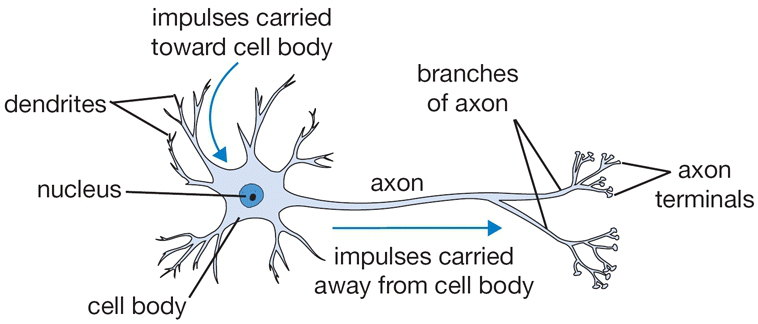
\includegraphics[width=\textwidth]{neuron.png}
  \column{0.5\textwidth}
  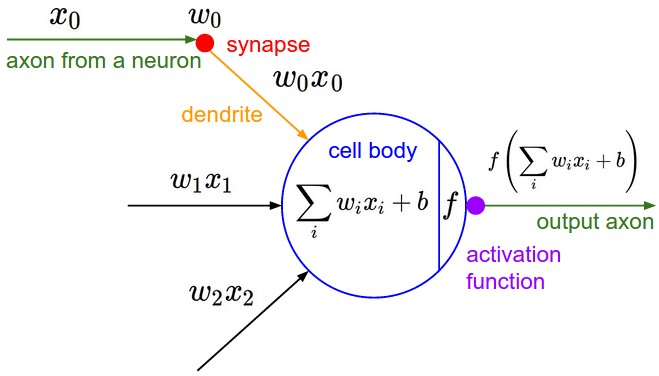
\includegraphics[width=\textwidth]{neuron_model.jpeg}
  \end{columns}
  \begin{itemize}
  \item A basic computational model of the biological model
  \item Single neuron as linear/logistic regression
  \end{itemize}
  \blfootnote{http://cs231n.github.io/neural-networks-1/}
\end{frame}

\begin{frame}
  \frametitle{Multi-Layer Perceptron}
  \begin{columns}
  \column{0.45\textwidth}
  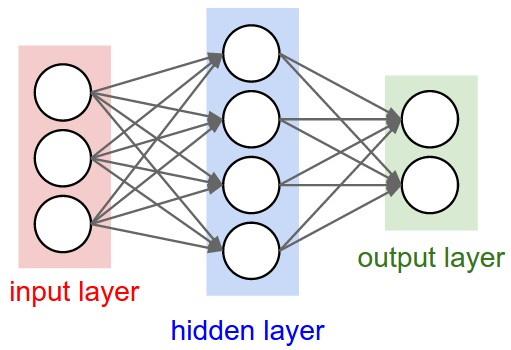
\includegraphics[height=1.3in]{neural_net.jpeg}
  \column{0.55\textwidth}
  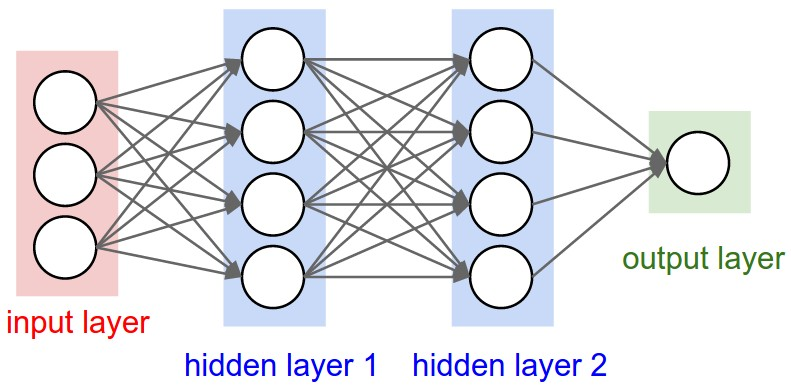
\includegraphics[height=1.3in]{neural_net2.jpeg}
  \end{columns}
  \begin{itemize}
  \item Neurons in an acyclic feed-forward graph
  \item Fully connected layers
  \item Each fully connected layer computation is a matrix multiplication,
    matrix addition and an activation function
  \end{itemize}
  \blfootnote{http://cs231n.github.io/neural-networks-1/}
\end{frame}

\begin{frame}
  \frametitle{What can an MLP learn?}
  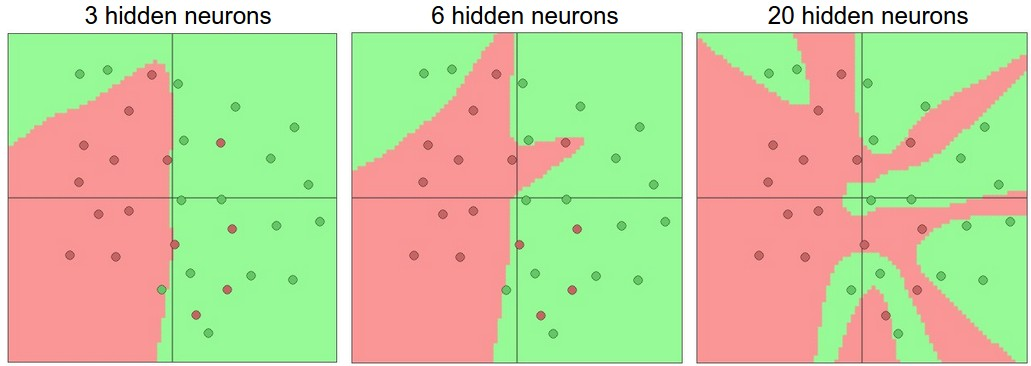
\includegraphics[width=\textwidth]{layer_sizes.jpeg}
  \begin{itemize}
  \item Neural Networks with at least one hidden layer are universal
    approximators\footnote{Approximation by superpositions of a sigmoidal function, by Cybenko G.}
  \item More neurons are expected to approximate better
  \end{itemize}
  \blfootnote{http://cs231n.github.io/neural-networks-1/}
\end{frame}

\section{Regularization}

\begin{frame}
  \frametitle{Regularization}
  \begin{itemize}
  \item Overfitting more probable with larger models
  \item Could be prevented by using a regularization term in the loss function
  \end{itemize}
\end{frame}

\begin{frame}
  \frametitle{Regularization}
  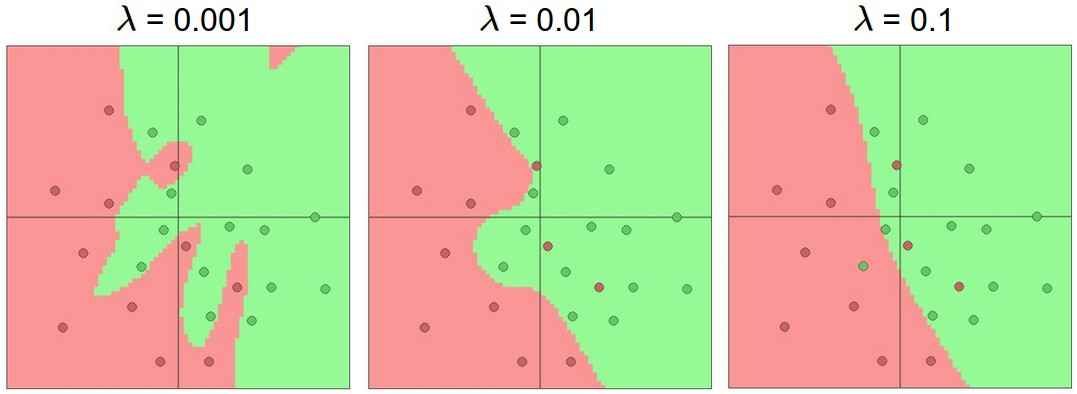
\includegraphics[width=\textwidth]{reg_strengths.jpeg}
  \begin{itemize}
  \item Use bigger networks but take measures to prevent overfitting
  \end{itemize}
  \blfootnote{http://cs231n.github.io/neural-networks-1/}
\end{frame}

\section{Convolution}

\begin{frame}
  \frametitle{Working with images}
  \begin{itemize}
  \item MLPs do not work well with images
  \item Hierarchy of local spatial features
  \item Extract these local spatial features through filters
  \end{itemize}
\end{frame}

\begin{frame}
  \frametitle{Convolution operation}

  \begin{equation*}
    s(t)=\int x(a)w(t-a)\, da
  \end{equation*}
  the operation is called \emph{convolution}. The convolution operation is typically denoted with $*$:
  \begin{equation*}
    s(t)=(x*w)(t)
  \end{equation*}
  In discrete form:
  \begin{equation*}
    s[t]=(x*w)(t)=\sum_{a=-\infty}^{\infty}x[a]w[t-a]
  \end{equation*}
\end{frame}

\begin{frame}
  \frametitle{2D convolution operation}

  \begin{equation*}
    s[i,j]=(I*K)[i,j]=\sum_{m}\sum_{n}I[m,n]K[i-m, j-n]
  \end{equation*}
  or equivalently:
  \begin{equation*}
    s[i,j]=(I*K)[i,j]=\sum_{m}\sum_{n}I[i-m, j-n]K[m,n]
  \end{equation*}
\end{frame}

\begin{frame}
  \frametitle{2D convolution operation}

 \begin{figure}
    \centering
    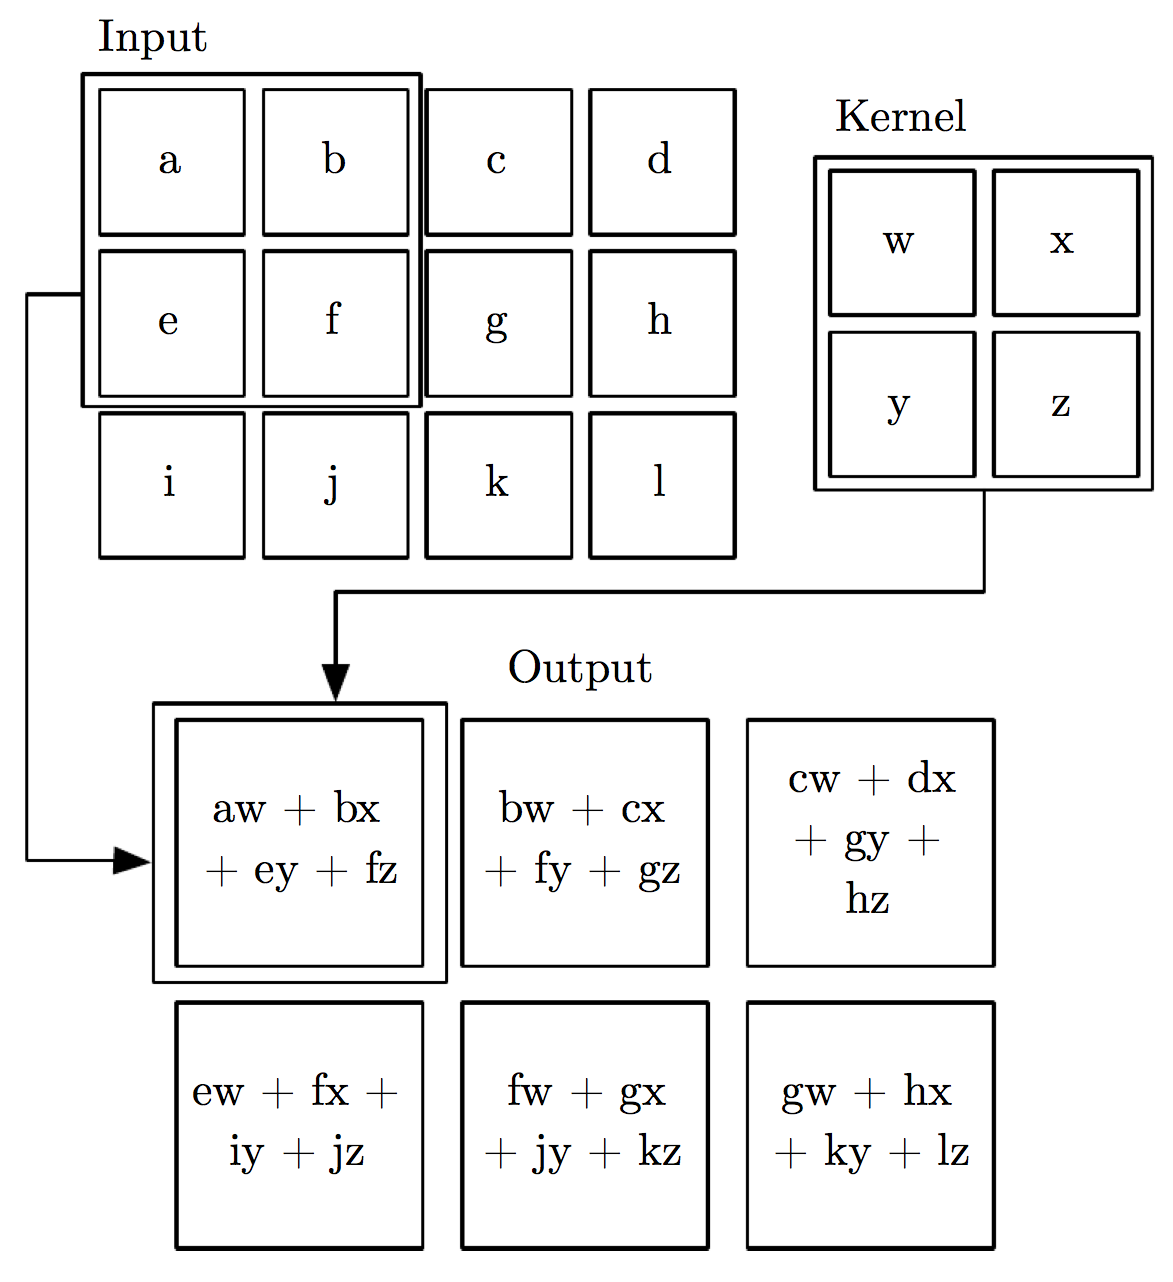
\includegraphics[width=0.55\textwidth]{convolution_operation.png}
  \end{figure}
\end{frame}

\section{Convolutional Neural Networks}

\begin{frame}
  \frametitle{LeNet-5}
  \begin{figure}[!htm]
    \centering
    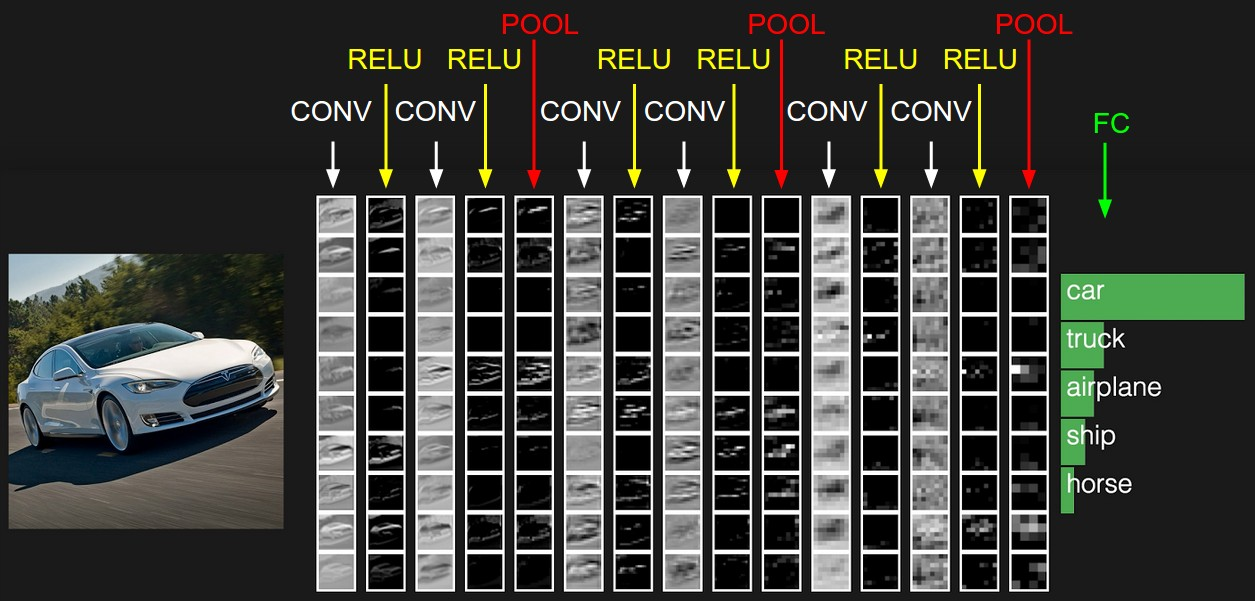
\includegraphics[width=0.8\textwidth]{convnet.jpeg}
  \end{figure}
\end{frame}

\begin{frame}
  \frametitle{MLP$\rightarrow$ConvNet}

  \begin{figure}[!htm]
    \centering
    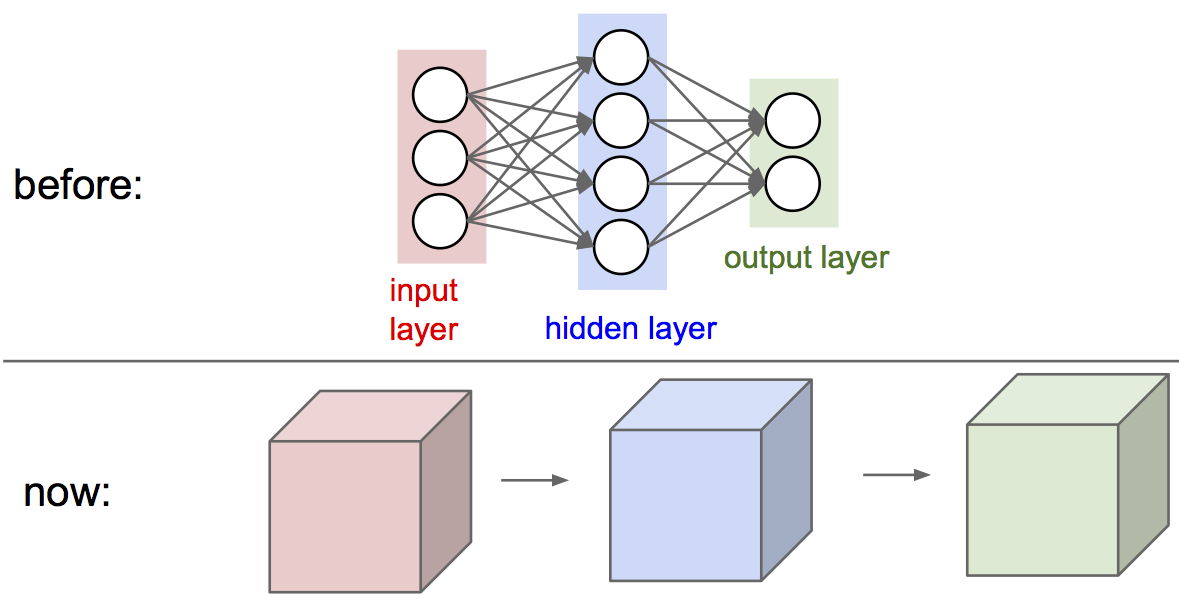
\includegraphics[width=0.8\textwidth]{convnet_gist.png}
  \end{figure}
\end{frame}

\begin{frame}
  \frametitle{Feature maps: activations of ConvNets}

  \begin{minipage}{0.48\textwidth}
    \begin{figure}[!htm]
      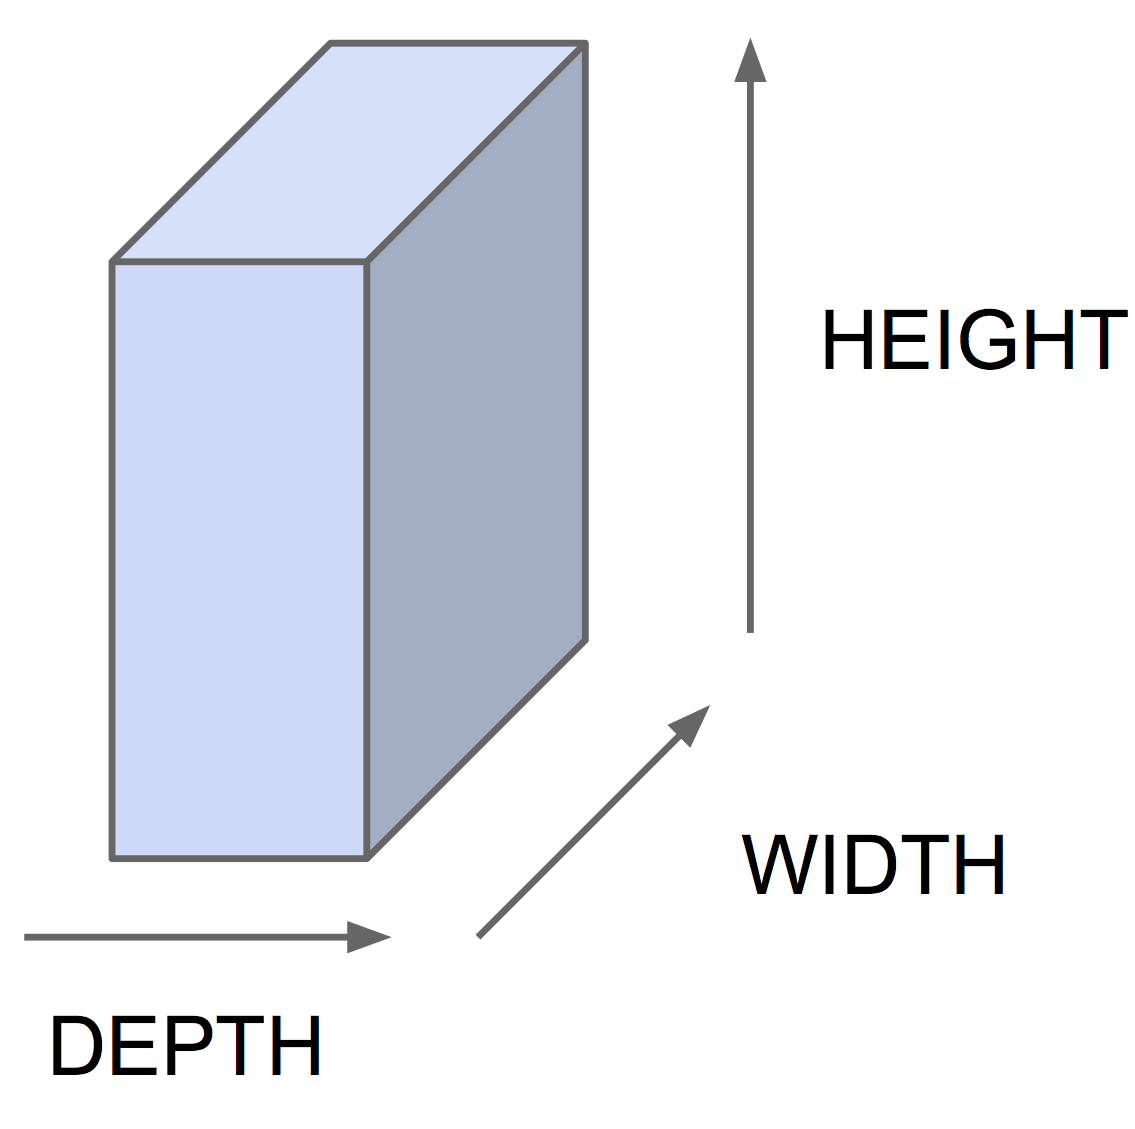
\includegraphics[width=0.8\textwidth]{feature_maps.png}
    \end{figure}
  \end{minipage}
  \begin{minipage}{0.48\textwidth}
    \begin{itemize}
      \item Network activations in ConvNets are \textbf{feature maps}.
      \item All ConvNets feature maps arranged in \textbf{3 dimensions}.
      \item Each feature maps has size of (HEIGHT, WIDTH)
      \item Input image can be a special kind of feature map (\emph{e.g.} color image is feature maps of some size with depth 3, one for each RGB channel).
    \end{itemize}
  \end{minipage}
\end{frame}

\begin{frame}
  \frametitle{Convolution Layer: simple cell}

  \begin{equation*}
    \mathbf{h}^{(k)}=f(\mathbf{x}*\mathbf{W}^{(k)}+b_{k})
  \end{equation*}

  \begin{itemize}
    \item Accepts a volume of size $W_{1}\times H_{1}\times D_{1}$
    \item Number of filters $K$ with shape $F\times F\times D_{1}$, stride $S$, amount of zero-padding $P$
    \item Produce a volume of size $W_{2}\times H_{2}\times D_{2}$ where
      \begin{align*}
        W_{2}&=(W_{1}-F+2P)/S+1 \\
        H_{2}&=(H_{1}-F+2P)/S+1 \\
        D_{2}&=K
      \end{align*}
  \end{itemize}

  \href{http://rt.dgyblog.com/res/dlworkshop/conv_demo.html}{Live Demo of convolution}
\end{frame}

\begin{frame}
  \frametitle{Pooling Layer: complex cell}

  \begin{figure}
    \centering
    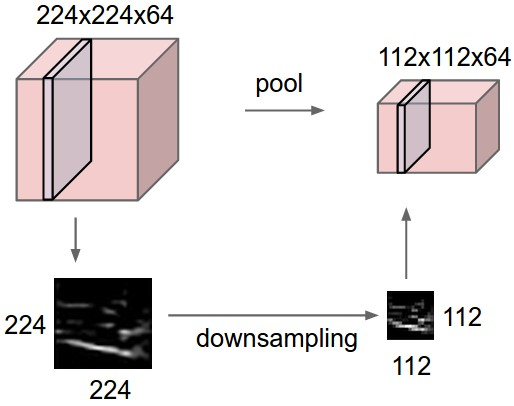
\includegraphics[width=0.25\textwidth]{pool.jpeg}\\
    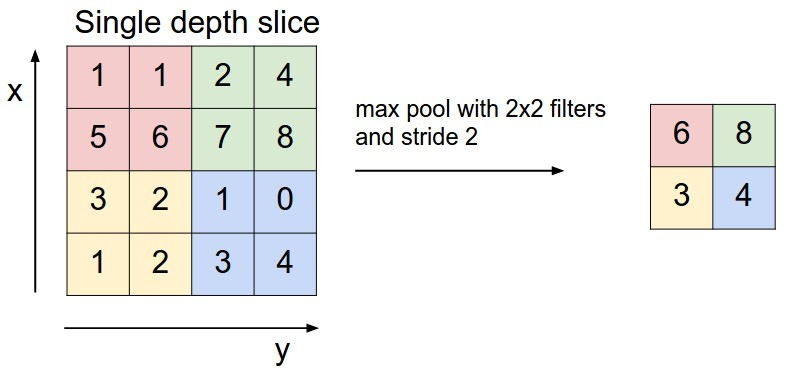
\includegraphics[width=0.5\textwidth]{maxpool.jpeg}
  \end{figure}
\end{frame}

\section*{Q\&A}

\begin{frame}
  \frametitle{Q\&A}
  \begin{figure}
    \centering
    
\includegraphics[width=0.7\textwidth]{convnet_how_to_work.png}
  \end{figure}
\end{frame}

\end{document}
%%% Local Variables:
%%% mode: latex
%%% TeX-master: t
%%% End:
